\documentclass[text05.tex]{subfiles}
\begin{document}
\subsubsection{\ruby{振動子}{しん|どう|し}}\label{vibrator}
\begin{table}[H]
  \begin{widerrows} 
    \begin{tabular}{|p{\colF}|p{\colG}|}	\hline
    \ruby{名称}{めい|しょう} & \ruby{振動子}{しん|どう|し}（しんどうし）\\ \hline
    \ruby{接続箇所}{せつ|ぞく|か|しょ} & デジタルコネクタ (3pin)\\ \hline
    \ruby{機能概要}{き|のう|がい|よう} & \ruby{振動}{しん|どう}モーターでふるえる\\ \hline
    \end{tabular}
  \end{widerrows} 
\end{table}

\begin{table}[H]
  \begin{widerrows} 
    \begin{tabular}{|p{\colF}|p{\colG}|}	\hline
    サンプルコードの場所 & 05/digout.hsp\\ \hline
    raspiへの入力 & なし\\ \hline
    raspiへの入力方法 & なし\\ \hline
    raspiからの出力 & \ruby{値}{あたい}が1のときふるえ、\ruby{値}{あたい}が0のとき動かない\\ \hline
    raspiからの出力方法 & gpio GPIO番号, パラメータ\\ \hline
    \end{tabular}
  \end{widerrows} 
\end{table}

\begin{table}[H]
  \begin{widerrows} 
    \begin{tabular}{|p{\colF}|p{\colG}|} \hline
    使い道 & \ruby{振動}{しん|どう}で何かが起きたことを伝える。目覚まし時計など。\\ \hline
    \ruby{注意事項}{ちゅう|い|じ|こう} & \ruby{振動}{しん|どう}している部分に\ruby{触}{ふ}って\ruby{怪我}{け|が}をしたり、\ruby{壊}{こわ}したりしないように注意\\ \hline
    \ruby{補足}{ほ|そく} & なし\\ \hline
    \end{tabular}
  \end{widerrows} 
\end{table}

\begin{figure}[H]
  \begin{widerrows}
    \begin{tabular}{|p{\colH}|p{\colI}|p{\colH}|p{\colI}|} \hline
    外観 & 
    \begin{minipage}[t]{\linewidth}
      \smallskip
        \centering
        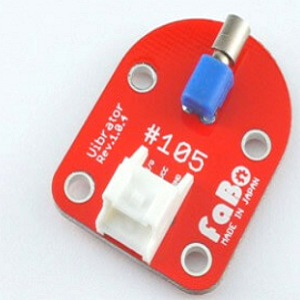
\includegraphics[width=0.5\linewidth]{../../asset/image/text05-img017.png}
        \caption{\ruby{振動子}{しん|どう|し}\hspace{0pt}}
        \smallskip
      \end{minipage} &
      回路記号 & 
      \begin{minipage}[t]{\linewidth}
      \smallskip
        \centering
        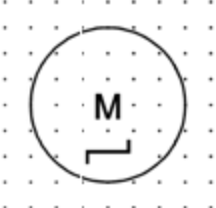
\includegraphics[width=0.5\linewidth]{../../asset/image/text05-img044.png}
        \caption{\ruby{振動子}{しん|どう|し}の回路図}
        \smallskip
      \end{minipage}\\ \hline
    \end{tabular}
  \end{widerrows} 
\end{figure}
\end{document}
